% if you want to include some content outside of frames also in slides, use \mode<
\mode<beamer|article>{
  \title{Publikace LaTeXových dokumentů na web pomocí TeX4ht a GitHub Actions}
  \author{Michal Hoftich}
  \maketitle
}

\begin{abstract}
Přednáška představí sadu šablon pro nástroj TeX4ht, který slouží k převodu
LaTeXových dokumentů do HTML. Tyto šablony výrazně usnadňují publikaci různých
typů dokumentů na webu a přinášejí moderní možnosti zpracování a automatizace.

První šablona je určena pro převod knižních dokumentů do webové podoby.
Umožňuje rozdělení textu do jednotlivých kapitol s automaticky generovanou
navigací a podporou responzivního designu, takže je výsledek dobře čitelný i na
mobilních zařízeních.

Druhá šablona slouží k tvorbě staticky generovaných blogů. Každý příspěvek je
psán jako samostatný LaTeXový dokument, který je pomocí TeX4ht převeden do
HTML. Následně jsou tyto články zpracovány statickým generátorem webů, jako je
například Jekyll, který se postará o sestavení celého blogu, vytvoření
rozcestníků, archivů a další navigace.

Třetí šablona je zaměřena na převod prezentací vytvořených v prostředí Beamer
do formy tzv. handoutů – přehledových materiálů pro posluchače. Výsledkem je
čitelný a dobře strukturovaný webový dokument vhodný pro sdílení po přednášce.

Všechny šablony jsou navrženy tak, aby fungovaly v rámci GitHub Actions. To
znamená, že dokumenty mohou být automaticky zkompilovány a publikovány online
pokaždé, když dojde ke změně v repozitáři. Tento přístup zajišťuje, že je
webová verze dokumentu vždy aktuální.
\end{abstract}

\tableofcontents

\section{Úvod}

Tato šablona je určena pro prezentace, které potřebují víc než jen snímky. Umožňuje vytvořit jak samotnou prezentaci, tak podrobný handout s poznámkami a komentáři. Všechny materiály tak lze generovat z jednoho zdrojového souboru – jak pro živou prezentaci, tak pro lidi, kteří se prezentace neúčastnili.

Obsahuje několik hlavních zdrojových souborů, každý s konkrétním účelem:

\begin{frame}[fragile]{Přehled souborů}
\begin{itemize}
\item \textbf{\texttt{slides.tex}}
\item \textbf{\texttt{handout.tex}}
\item \textbf{\texttt{presentation.tex}}
\item \textbf{\texttt{preamble.tex}}
\item \textbf{\texttt{config.cfg}}
\end{itemize}
\end{frame}

\begin{itemize}
\item \textbf{\texttt{slides.tex}} – Tento soubor slouží ke generování hlavní prezentace ve formátu Beamer. Obsahuje to, co se zobrazuje během přednášky.

\item \textbf{\texttt{handout.tex}} – Handoutová verze prezentace, formátovaná jako standardní článek. Kromě obsahu viditelného na snímcích obsahuje i doplňující poznámky a komentáře, které se v samotné prezentaci nezobrazují. Tento soubor je určen ke sdílení po skončení prezentace a měl by být samostatně použitelný i pro čtenáře, kteří prezentaci neviděli.

\item \textbf{\texttt{presentation.tex}} – Obsahuje celý zdrojový text prezentace. Obsah uvnitř prostředí \verb|\begin{frame}...\end{frame}| se zahrnuje jak do \texttt{slides.tex}, tak do \texttt{handout.tex}. Text mimo prostředí frame se v prezentaci nezobrazí, ale je součástí handoutu. To umožňuje doplnit prezentaci o podrobnější komentáře, vysvětlení nebo poznámky.

\item \textbf{preamble.tex} – Obsahuje balíčky a definice příkazů používané v prezentaci.

\item \textbf{config.cfg} – Konfigurační soubor pro \TeX4ht. Například zde můžete upravit CSS styly použité ve webové verzi dokumentu nebo redefinice \LaTeX{}ových příkazů.
\end{itemize}

Tyto soubory si můžete upravit podle svých potřeb. Minimálně je vhodné nahradit obsah \texttt{presentation.tex} vlastním textem a případně upravit \texttt{preamble.tex}, pokud potřebujete přidat další balíčky nebo příkazy.

\section{Základní použití}


\begin{frame}[fragile]{Vytvoření nového GitHub repozitáře}
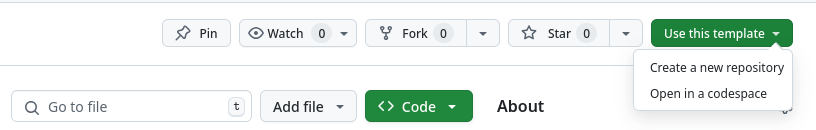
\includegraphics[width=\textwidth]{img/template-use.png}
\end{frame}

Chcete-li začít s vlastní prezentací podle této šablony, klikněte na tlačítko "Use this template" na stránce GitHub repozitáře. Tím se ve vašem účtu vytvoří nový repozitář se stejnou strukturou a soubory. Poté jej můžete naklonovat, upravit obsah a začít vytvářet vlastní snímky a handouty.

\begin{frame}[fragile]{Použití prostředí frame a komentáře v handoutu}

\begin{block}{}
Základní syntaxe dokumentu používaného v souboru \verb|presentation.tex| vypadá následovně:
\end{block}

\begin{likeverbatim}\verb|\begin{frame}{Název snímku}|\
\verb|obsah snímku...|\
\verb|\end|\verb|{frame}|\
\vspace{1em}
\verb|Komentář, který bude zahrnut pouze v handoutu|
\end{likeverbatim}

\end{frame}

Například zdrojový kód jednoho z předchozích snímků vypadá takto:

\verb|\begin|\verb|{frame}[fragile]{Přehled souborů}|
\begin{verbatim}
\begin{itemize}
\item \textbf{\texttt{slides.tex}}
\item \textbf{\texttt{handout.tex}}
\item \textbf{\texttt{presentation.tex}}
\item \textbf{\texttt{preamble.tex}}
\end{itemize}
\end{verbatim}
\verb|\end|\verb|{frame}|

\begin{verbatim}
\begin{itemize}
\item \textbf{\texttt{slides.tex}} – Tento soubor slouží ke generování hlavní
prezentace ve formátu Beamer. Obsahuje to, co se zobrazuje během přednášky.
\end{itemize}
\end{verbatim}

Obsah uvnitř bloku \verb|\begin|\verb|{frame}...\end|\verb|{frame}| se zahrne
do prezentace i handoutu, ale prostředí \texttt{itemize}, které následuje za
ním, se zobrazí pouze v handoutu.

\begin{frame}[fragile]{Sdílený obsah mimo prostředí frame}

\begin{verbatim}
\mode<beamer|article>{
\title{Strukturovaná šablona prezentace}
\author{Michal Hoftich}
\maketitle
}
\end{verbatim}
\end{frame}

Příkaz \verb+\mode<beamer|article>{...}+ umožňuje zahrnout obsah, který se má
zobrazit jak v prezentaci, tak v handoutu. To se může hodit například pro název
prezentace nebo obsah prezentace.

\section{Kompilace prezentace}

\begin{frame}[fragile]{Kompilace do PDF}

Prezentaci nebo handout můžete zkompilovat do PDF pomocí LuaLaTeXu těmito příkazy:

\begin{verbatim}
$ lualatex slides.tex
$ lualatex handout.tex
\end{verbatim}
\end{frame}



Výstupní soubory můžete kompilovat v libovolné standardní distribuci \LaTeX{}u, která obsahuje Beamer a potřebné balíčky.

\begin{frame}[fragile]{HTML verze}
Pro převod prezentace do formátu HTML použijte nástroj \href{https://www.tug.org/tex4ht/}{\TeX4ht}.
\begin{verbatim}
$ make4ht -l handout.tex\end{verbatim}

Přepínač \verb|-l| zajistí použití Lua\LaTeX{}u jako překladače.
\end{frame}

HTML verze se generuje z handoutu ve stylu článku, nikoliv z Beamer prezentace.
To ji činí vhodnější pro webové publikování nebo dlouhodobé sdílení, protože
obsahuje všechny vysvětlivky a není závislá na rozvržení snímků.

section{Automatické generování HTML výstupu}

Tato část vysvětluje, jak se používají \href{https://docs.github.com/en/actions/writing-workflows/quickstart}{GitHub Actions} k automatickému generování a publikování HTML verze materiálů při každém pushnutí změn do větve \texttt{main}.

Výstup je vytvářen pomocí \texttt{make4ht} a publikován do větve \texttt{gh-pages}, což usnadňuje sdílení webové verze prezentace.

\begin{frame}[fragile]{Přehled GitHub Actions}
Klíčové části workflow pro sestavení a publikování HTML:

\begin{verbatim}

    name: Spuštění make4ht
    uses: xu-cheng/texlive-action/full@v1
    with:
      run: |
      make4ht -lj index -a debug -d out handout.tex

    name: Publikování webových stránek
    uses: peaceiris/actions-gh-pages@v3
    with:
      github_token: ${{ secrets.GITHUB_TOKEN }}
      publish_dir: ./out
\end{verbatim}

\end{frame}

Workflow je definován v souboru \texttt{.github/workflows/main.yml}.
Tento soubor můžete upravit pro přizpůsobení procesu sestavení, například změnou parametrů pro \texttt{make4ht}.

Používají se dvě GitHub Actions: \href{https://github.com/xu-cheng/texlive-action}{xu-cheng/texlive-action}
a \href{https://github.com/peaceiris/actions-gh-pages}{peaceiris/actions-gh-pages}.
První umožňuje používat libovolný příkaz dostupný v TeX Live instalaci, jako \texttt{make4ht} nebo \texttt{lualatex}.
Druhá publikuje obsah zadaného adresáře do větve \texttt{gh-pages} vašeho repozitáře,
kterou GitHub Pages používá pro zobrazování statického obsahu.

\begin{frame}[fragile]{Automatické sestavení HTML}
Změny pushnuté do větve \texttt{main} spustí GitHub Actions workflow, který:

\begin{itemize}
\item Zkompiluje \texttt{handout.tex} do HTML pomocí \texttt{make4ht}
\item Publikuje výstup do větve \texttt{gh-pages}
\end{itemize}

Použitý příkaz je:

\begin{verbatim}
make4ht -lj index -a debug -d out handout.tex
\end{verbatim}
\end{frame}

Tento příkaz vytvoří HTML soubory v adresáři \texttt{out/}, které jsou následně publikovány
pomocí akce \texttt{peaceiris/actions-gh-pages}, specifikované nastavením
\texttt{publish_dir}.

\begin{frame}[fragile]{Proč \texttt{-j index}?}
\begin{itemize}
\item Volba \texttt{-lj index} je zkratka pro \texttt{-l -j index}
\item Volba \texttt{-j index} nastaví název výstupního HTML souboru na \texttt{index.html}
\item To umožňuje používat čisté URL adresy jako:

\begin{verbatim}
https://username.github.io/repo/
\end{verbatim}

\end{itemize}
\end{frame}

Není potřeba v URL specifikovat název souboru - GitHub Pages
automaticky hledá soubor \texttt{index.html}. Toto usnadňuje sdílení
prezentace a pomáhá předejít nefunkčním odkazům kvůli neshodě názvů souborů.

Například tato prezentace je dostupná na: \url{https://michal-h21.github.io/tex4ht-presentation/}.

\section{Github Pages}

\begin{frame}[fragile]{Rozhraní Github Actions}
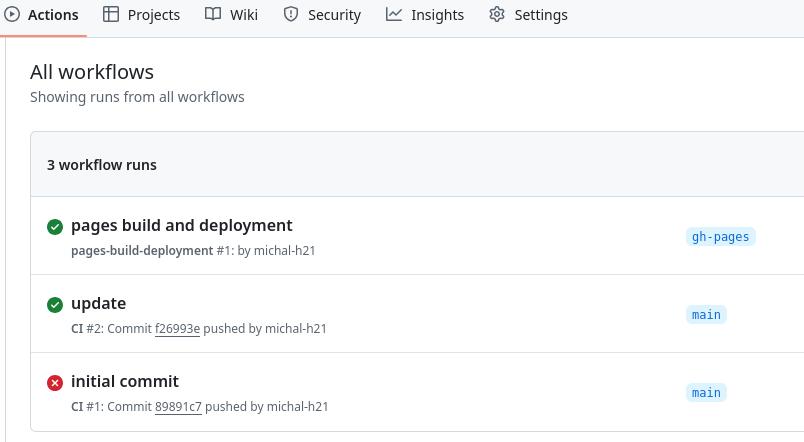
\includegraphics[width=\textwidth]{img/github-actions.png}
\end{frame}

Po pushnutí změn do větve \texttt{main} můžete zkontrolovat záložku \texttt{Actions} ve vašem
Github repozitáři. Zobrazuje stav workflow, včetně informace o úspěšném dokončení nebo případných chybách.

\begin{frame}[fragile]{Chyby}
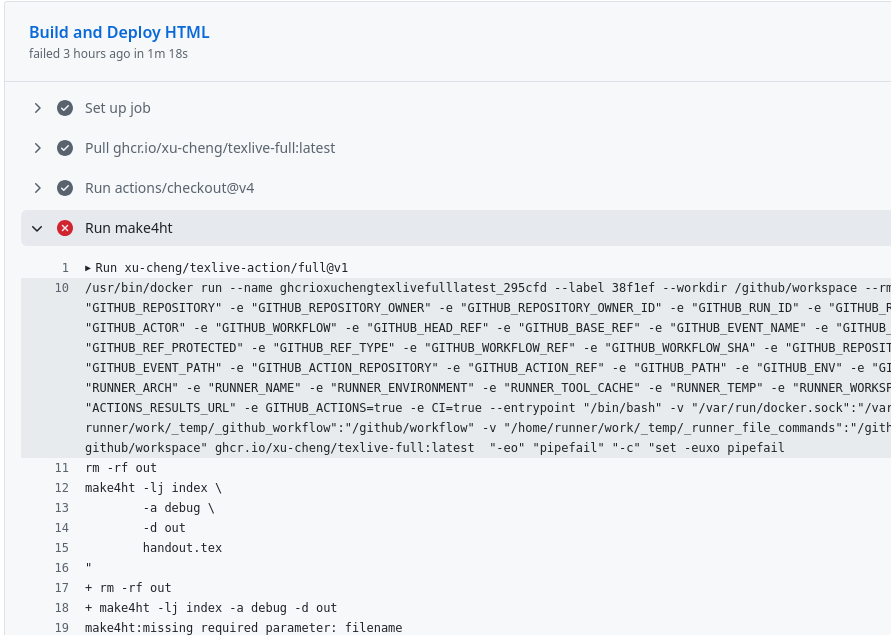
\includegraphics[width=\textwidth]{img/github-error.png}
\end{frame}

Můžete také zkontrolovat logy běhu workflow, abyste viděli, co se pokazilo.
Pokud narazíte na chybu, bude zobrazena v logu a můžete tyto informace
použít k řešení problému.

V tomto případě byl nesprávný název TeX souboru. Musel jsem opravit název souboru v YAML souboru GitHub Actions.

\begin{frame}[fragile]{Nastavení Github Pages}
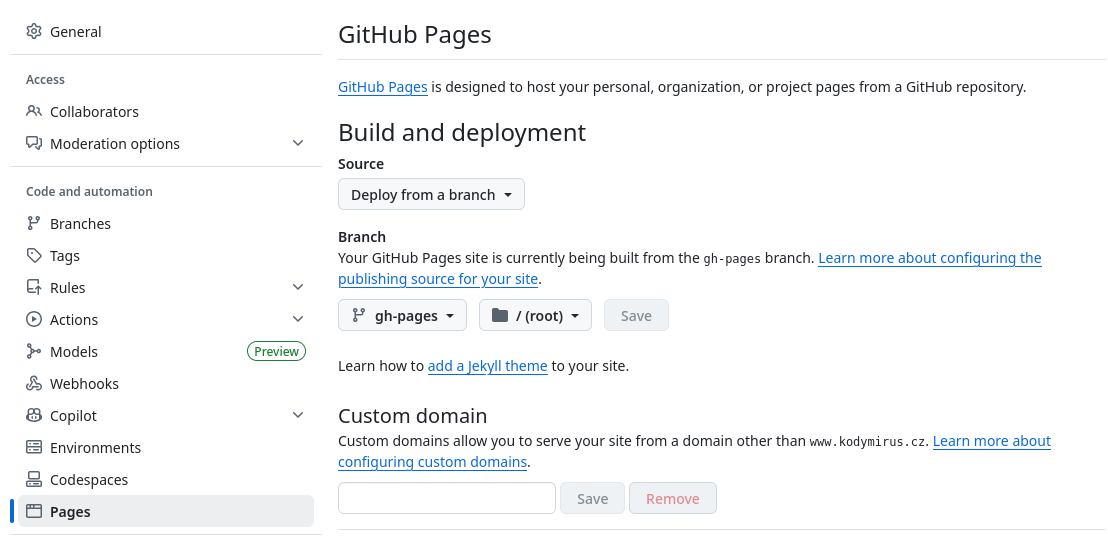
\includegraphics[width=\textwidth]{img/github-pages.png}
\end{frame}

Po úspěšném dokončení workflow můžete nastavit GitHub Pages pro zobrazování obsahu větve \texttt{gh-pages}.

Všechny výstupní soubory vytvořené pomocí \texttt{make4ht} budou dostupné na webu.
Budou přístupné na adrese:
\verb|https://username.github.io/repo/|,
kde \texttt{username} je vaše GitHub uživatelské jméno a \texttt{repo} je název vašeho repozitáře.
